\input{../YKY-preamble.tex}

\usepackage{color}
\usepackage{mathtools}
\usepackage{hyperref}

% \usepackage[backend=biber,style=numeric]{biblatex}
% \bibliography{../AGI-book}
% \renewcommand*{\bibfont}{\footnotesize}

\usepackage{graphicx} % Allows including images
\usepackage{tikz-cd}
\usepackage{tikz}
\usepackage[export]{adjustbox}% http://ctan.org/pkg/adjustbox
\usepackage{verbatim} % for comments
% \usepackage{newtxtext,newtxmath}	% Times New Roman font

% \numberwithin{equation}{subsection}

\newcommand{\underdash}[1]{%
	\tikz[baseline=(toUnderline.base)]{
		\node[inner sep=1pt,outer sep=10pt] (toUnderline) {#1};
		\draw[dashed] ([yshift=-0pt]toUnderline.south west) -- ([yshift=-0pt]toUnderline.south east);
	}%
}%

\DeclareSymbolFont{symbolsC}{U}{txsyc}{m}{n}
\DeclareMathSymbol{\strictif}{\mathrel}{symbolsC}{74}

\newcommand{\highlight}[1]{\colorbox{pink}{$\displaystyle #1$}}

\newcommand{\emp}[1]{{\color{violet}\textbf{#1}}}
\newcommand*\confoundFace{$\vcenter{\hbox{\includegraphics[scale=0.2]{../2020/../confounded-face.jpg}}}$}
\newcommand{\underconst}{\includegraphics[scale=0.5]{../2020/UnderConst.png}}
\newcommand{\witness}{\scalebox{0.6}{$\blacksquare$}}
% \newcommand{\Heytingarrow}{\mathrel{-}\mathrel{\triangleright}}
\providecommand\Heytingarrow{\relbar\joinrel\mathrel{\vcenter{\hbox{\scalebox{0.75}{$\rhd$}}}}}

\begin{document}

\title{\bfseries\color{blue}{\Huge AGI standard model}\\ --- a proposal}
\author{YKY} % Your name
%\institute[] % Your institution as it will appear on the bottom of every slide, may be shorthand to save space
%{
%Independent researcher, Hong Kong \\ % Your institution for the title page
%\medskip
%\textit{generic.intelligence@gmail.com} % Your email address
%}
\date{\today} % Date, can be changed to a custom date

\maketitle

% \vspace*{0.5cm}
% 多谢 支持 \smiley

\setcounter{section}{-1}
\section{Introduction}

The ``standard model'' is a way of thinking, that may help us better understand the general theory of AGI systems.

The essence of the standard model is just to identify a \textbf{Working Memory} or ``state'' of the AGI system.

One benefit of our theory is that it relates Transformers / BERT / GPT to AGI systems.  These language models are phenomenally intelligent, yet many people criticize them as not ``truly'' intelligent.  The standard model suggests that they are indeed linked to AGI.  There are other benefits.

\section{Reinforcement learning}

The simplest form of a \textbf{dynamical system}:

When we add an ``action'' or ``control'' variable to it, it becomes the simplest \textbf{control system}:

which is the setting for Dynamic Programming or Reinforcement Learning.

\section{Standard model}

\begin{equation}
\vcenter{\hbox{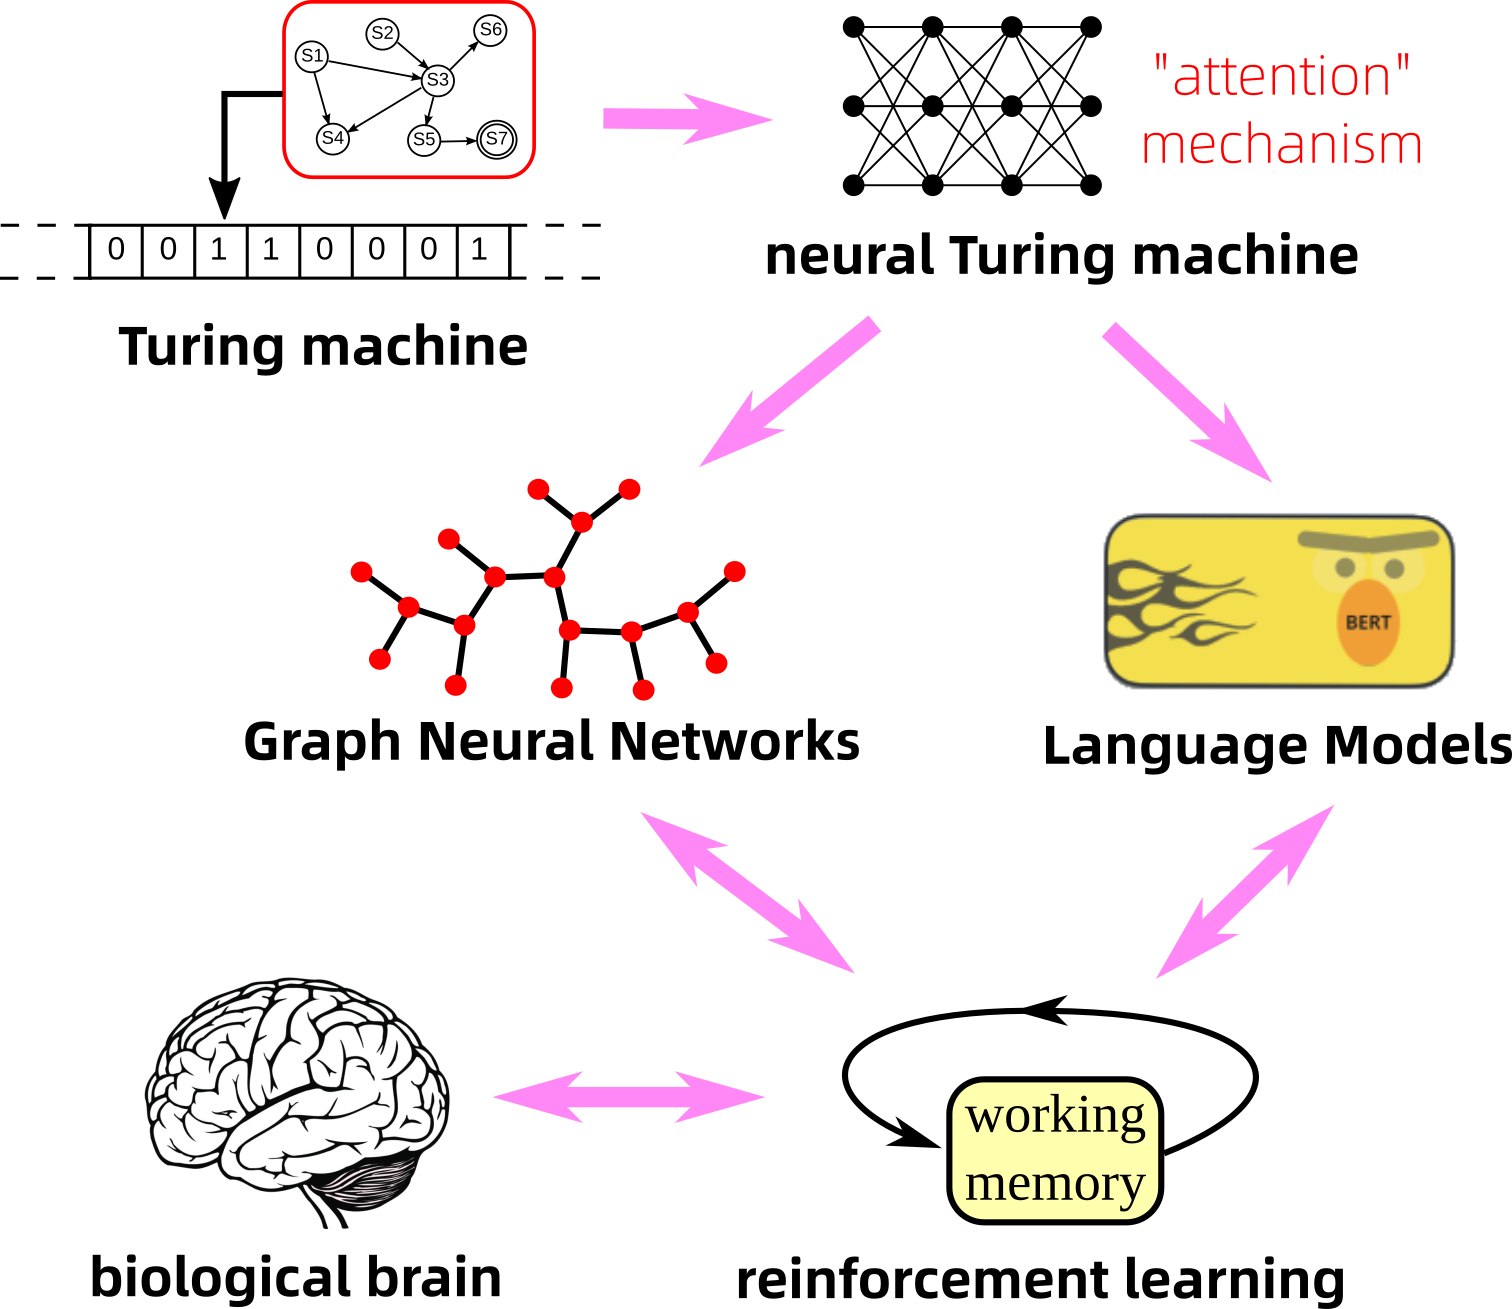
\includegraphics[scale=0.9]{AGI-standard-model.png}}}
\end{equation}

\section{Neural Turing Machine and BERT}

The \textbf{attention mechanism} was first proposed in the ``\textbf{Neural Turing Machine}'' paper by Graves et al.

\section{Relation to the biological brain}

The prefrontal cortex maintains a number of ``thoughts'' with sub-populations or, perhaps, with \textbf{micro-columns}.  These activated sub-populations are in competition with each other, through \textbf{lateral inhibition}.  The thought(s) that win are the thoughts we retain -- they ``make sense''.

\section{Abductive reasoning}

Abductive reasoning is basically just \textbf{bidirectional} inference.

When a system has both forward and backward connections, it forms a loop and its dynamics is likely to produce ``resonance''.  This harks back to the ART (Adaptive Resonance Theory) proposed by Grossberg and Carpenter beginning in the 1980s.

Such resonance behavior can be viewed as the system seeking to minimize an energy, ie, trying to find the ``best explanation'' to a set of facts.  

\section{Dealing with assumptions}

Example of an assumption:  ``If I play move $x$ now, I will checkmate in 3 moves".

Suppose $M, N$ are proofs of $M: \phi \rightarrow \psi$ and $N: \phi$.  Then the proof of $\psi$ would be the application of $M$ to $N$, denoted as $@(M, N)$ or simply $M N$.

The assumption rule (Ax):
\begin{equation}
\Gamma, \phi \vdash \phi \qquad (\mbox{Ax})
\end{equation}
for example can be written as:
\begin{equation}
x : \phi, \; y : \psi \vdash x : \phi \qquad (\mbox{Ax})
\end{equation}
which is why we say that an assumption is a \textbf{$\lambda$-variable}.  

\textbf{Discharging} an assumption (ie, using the $\rightarrow$I rule) results in a $\lambda$-term.

An AGI needs the ability to place an implication $\phi \rightarrow \psi$ into working memory, and to prove it using the ($\rightarrow$ I) rule, ie, by making an assumption.

\end{document}
